\begin{figure}[!htbp]%
\centering
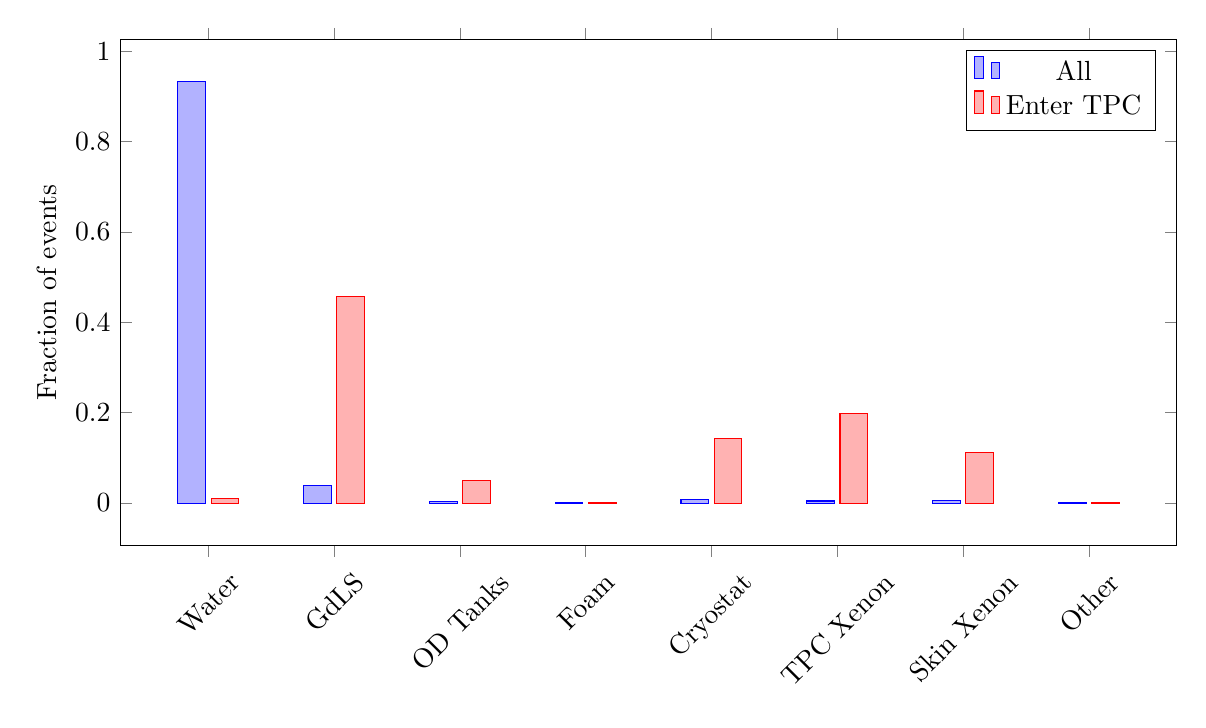
\begin{tikzpicture}  
\begin{axis}  
[  
    width=15cm,
    height=8cm,
    ybar,
    %enlargelimits=0.15,
    %legend style={at={(0.4,-0.25)},
    %  anchor=north,legend columns=-1},     
    ylabel={Fraction of events}, 
    symbolic x coords={Water, GdLS, OD Tanks, Foam, Cryostat, TPC Xenon, Skin Xenon, Other},  
    xtick=data,  
    xticklabel style={rotate=45},
    %nodes near coords,  
    %nodes near coords align={vertical},  
    ]  
\addplot coordinates {(Water, 0.9322466611383653)
                        (GdLS, 0.03855767704533553)
                        (OD Tanks, 0.00410320616756687)
                        (Foam, 6.972186908013119e-05)
                        (Cryostat, 0.007627869166170949)
                        (TPC Xenon, 0.00464169634790916)
                        (Skin Xenon, 0.00490723282802285)
                        (Other, 4.153643264348242e-05)};
\addplot coordinates {(Water, 0.009676137378112347)
                      (GdLS, 0.4578022497019404)
                      (OD Tanks, 0.049714035582843284)
                      (Foam, 0.0014830984374190055)
                      (Cryostat, 0.14357832775611526)
                      (TPC Xenon, 0.19879854627555105)
                      (Skin Xenon, 0.11225759260005874)
                      (Other, 0.00010367290047977514)}; 
  \legend{All, Enter TPC};
\end{axis}  
\end{tikzpicture}  
    \caption{Fraction of background neutrons expected to get captured in each detector volume for all background neutrons and for neutrons that \textbf{SS} in the TPC Xenon.}
    \label{fig:simulated_neutron_capture_volumes}
\end{figure}

